% Created 2016-01-08 Fri 16:42
\documentclass[presentation]{beamer}
\usepackage[utf8]{inputenc}
\usepackage[T1]{fontenc}
\usepackage{fixltx2e}
\usepackage{graphicx}
\usepackage{grffile}
\usepackage{longtable}
\usepackage{wrapfig}
\usepackage{rotating}
\usepackage[normalem]{ulem}
\usepackage{amsmath}
\usepackage{textcomp}
\usepackage{amssymb}
\usepackage{capt-of}
\usepackage{hyperref}
\usepackage{minted}
\usepackage{tikz}
\usepgflibrary{shapes.geometric}
\usetikzlibrary{calc}
\usetikzlibrary{positioning}
\usetheme{EPCC}
\author{Lawrence Mitchell\thanks{lawrence.mitchell@ed.ac.uk} (EPCC), Florian Rathgeber, Graham Markall, Nicolas Loriant, Carlo Bertolli, David Ham, Paul Kelly (Imperial College), Gihan Mudalige, Mike Giles (Oxford)}
\date{Tuesday 18th March 2013}
\title{PyOP2: a framework for fast, unstructured mesh computations}
\hypersetup{
 pdfauthor={Lawrence Mitchell\thanks{lawrence.mitchell@ed.ac.uk} (EPCC), Florian Rathgeber, Graham Markall, Nicolas Loriant, Carlo Bertolli, David Ham, Paul Kelly (Imperial College), Gihan Mudalige, Mike Giles (Oxford)},
 pdftitle={PyOP2: a framework for fast, unstructured mesh computations},
 pdfkeywords={},
 pdfsubject={},
 pdfcreator={Emacs 24.5.1 (Org mode 8.3.2)}, 
 pdflang={English}}
\begin{document}

\maketitle
\begin{frame}{Outline}
\tableofcontents
\end{frame}


\section{Overview}
\label{sec:orgheadline5}

\begin{frame}[label={sec:orgheadline1}]{Hardware zoo}
\begin{itemize}
\item Multicore CPU
\item Manycore CPU (phi)
\item GPU
\item All tied together with a network
\end{itemize}
\end{frame}

\begin{frame}[label={sec:orgheadline2}]{Performance portability}
\begin{itemize}
\item What if we want our code to run on different hardware?
\item Can we avoid porting to new hardware?
\end{itemize}
\end{frame}

\begin{frame}[label={sec:orgheadline3}]{Premise}
\begin{itemize}
\item Current typical codes intimately tie numerics to implementation
\begin{itemize}
\item Developers must be experts in multiple domains
\end{itemize}
\item Can we design abstractions that separate numerics from
implementation?
\begin{itemize}
\item and allow us to automatically \emph{generate} high-performance code
\end{itemize}
\item Not an auto-parallelising compiler (too much work)
\end{itemize}
\end{frame}

\begin{frame}[label={sec:orgheadline4}]{Problem domain}
\begin{itemize}
\item unstructured mesh computations
\item typically have some elementary operation we wish to apply over all
entities in a mesh
\end{itemize}
\end{frame}

\section{The OP2 abstraction}
\label{sec:orgheadline13}
\begin{frame}[label={sec:orgheadline6}]{Data types}
\begin{itemize}
\item \emph{Sets} of mesh entities
\begin{itemize}
\item vertices
\item facets
\item elements
\item degrees of freedom
\item \ldots{}
\end{itemize}
\end{itemize}

\begin{center}
\only<1>{\documentclass{article}
\usepackage{tikz}
\usetikzlibrary{arrows}
\begin{document}

\tikzstyle{n}=[circle, fill, minimum size=4pt, inner sep=0pt]
\pagestyle{empty}
\begin{tikzpicture}[scale=8]
\node[n] (0) at (0, 0) {};
\node[n] (1) at (1, 0) {};
\node[n] (2) at (0, 1) {};
\node[n] (3) at (1, 1) {};
\node[n] (4) at (0.1, 0) {};
\node[n] (5) at (0.2, 0) {};
\node[n] (6) at (0.3, 0) {};
\node[n] (7) at (0.4, 0) {};
\node[n] (8) at (0.5, 0) {};
\node[n] (9) at (0.6, 0) {};
\node[n] (10) at (0.7, 0) {};
\node[n] (11) at (0.8, 0) {};
\node[n] (12) at (0.9, 0) {};
\node[n] (13) at (0.1, 1) {};
\node[n] (14) at (0.2, 1) {};
\node[n] (15) at (0.3, 1) {};
\node[n] (16) at (0.4, 1) {};
\node[n] (17) at (0.5, 1) {};
\node[n] (18) at (0.6, 1) {};
\node[n] (19) at (0.7, 1) {};
\node[n] (20) at (0.8, 1) {};
\node[n] (21) at (0.9, 1) {};
\node[n] (22) at (0, 0.1) {};
\node[n] (23) at (0, 0.2) {};
\node[n] (24) at (0, 0.3) {};
\node[n] (25) at (0, 0.4) {};
\node[n] (26) at (0, 0.5) {};
\node[n] (27) at (0, 0.6) {};
\node[n] (28) at (0, 0.7) {};
\node[n] (29) at (0, 0.8) {};
\node[n] (30) at (0, 0.9) {};
\node[n] (31) at (1, 0.1) {};
\node[n] (32) at (1, 0.2) {};
\node[n] (33) at (1, 0.3) {};
\node[n] (34) at (1, 0.4) {};
\node[n] (35) at (1, 0.5) {};
\node[n] (36) at (1, 0.6) {};
\node[n] (37) at (1, 0.7) {};
\node[n] (38) at (1, 0.8) {};
\node[n] (39) at (1, 0.9) {};
\node[n] (40) at (0.1, 0.1) {};
\node[n] (41) at (0.1, 0.2) {};
\node[n] (42) at (0.1, 0.3) {};
\node[n] (43) at (0.1, 0.4) {};
\node[n] (44) at (0.1, 0.5) {};
\node[n] (45) at (0.1, 0.6) {};
\node[n] (46) at (0.1, 0.7) {};
\node[n] (47) at (0.1, 0.8) {};
\node[n] (48) at (0.1, 0.9) {};
\node[n] (49) at (0.2, 0.1) {};
\node[n] (50) at (0.2, 0.2) {};
\node[n] (51) at (0.2, 0.3) {};
\node[n] (52) at (0.2, 0.4) {};
\node[n] (53) at (0.2, 0.5) {};
\node[n] (54) at (0.2, 0.6) {};
\node[n] (55) at (0.2, 0.7) {};
\node[n] (56) at (0.2, 0.8) {};
\node[n] (57) at (0.2, 0.9) {};
\node[n] (58) at (0.3, 0.1) {};
\node[n] (59) at (0.3, 0.2) {};
\node[n] (60) at (0.3, 0.3) {};
\node[n] (61) at (0.3, 0.4) {};
\node[n] (62) at (0.3, 0.5) {};
\node[n] (63) at (0.3, 0.6) {};
\node[n] (64) at (0.3, 0.7) {};
\node[n] (65) at (0.3, 0.8) {};
\node[n] (66) at (0.3, 0.9) {};
\node[n] (67) at (0.4, 0.1) {};
\node[n] (68) at (0.4, 0.2) {};
\node[n] (69) at (0.4, 0.3) {};
\node[n] (70) at (0.4, 0.4) {};
\node[n] (71) at (0.4, 0.5) {};
\node[n] (72) at (0.4, 0.6) {};
\node[n] (73) at (0.4, 0.7) {};
\node[n] (74) at (0.4, 0.8) {};
\node[n] (75) at (0.4, 0.9) {};
\node[n] (76) at (0.5, 0.1) {};
\node[n] (77) at (0.5, 0.2) {};
\node[n] (78) at (0.5, 0.3) {};
\node[n] (79) at (0.5, 0.4) {};
\node[n] (80) at (0.5, 0.5) {};
\node[n] (81) at (0.5, 0.6) {};
\node[n] (82) at (0.5, 0.7) {};
\node[n] (83) at (0.5, 0.8) {};
\node[n] (84) at (0.5, 0.9) {};
\node[n] (85) at (0.6, 0.1) {};
\node[n] (86) at (0.6, 0.2) {};
\node[n] (87) at (0.6, 0.3) {};
\node[n] (88) at (0.6, 0.4) {};
\node[n] (89) at (0.6, 0.5) {};
\node[n] (90) at (0.6, 0.6) {};
\node[n] (91) at (0.6, 0.7) {};
\node[n] (92) at (0.6, 0.8) {};
\node[n] (93) at (0.6, 0.9) {};
\node[n] (94) at (0.7, 0.1) {};
\node[n] (95) at (0.7, 0.2) {};
\node[n] (96) at (0.7, 0.3) {};
\node[n] (97) at (0.7, 0.4) {};
\node[n] (98) at (0.7, 0.5) {};
\node[n] (99) at (0.7, 0.6) {};
\node[n] (100) at (0.7, 0.7) {};
\node[n] (101) at (0.7, 0.8) {};
\node[n] (102) at (0.7, 0.9) {};
\node[n] (103) at (0.8, 0.1) {};
\node[n] (104) at (0.8, 0.2) {};
\node[n] (105) at (0.8, 0.3) {};
\node[n] (106) at (0.8, 0.4) {};
\node[n] (107) at (0.8, 0.5) {};
\node[n] (108) at (0.8, 0.6) {};
\node[n] (109) at (0.8, 0.7) {};
\node[n] (110) at (0.8, 0.8) {};
\node[n] (111) at (0.8, 0.9) {};
\node[n] (112) at (0.9, 0.1) {};
\node[n] (113) at (0.9, 0.2) {};
\node[n] (114) at (0.9, 0.3) {};
\node[n] (115) at (0.9, 0.4) {};
\node[n] (116) at (0.9, 0.5) {};
\node[n] (117) at (0.9, 0.6) {};
\node[n] (118) at (0.9, 0.7) {};
\node[n] (119) at (0.9, 0.8) {};
\node[n] (120) at (0.9, 0.9) {};
\draw (0) -- (4) -- (40) -- (0);
\draw (0) -- (40) -- (22) -- (0);
\draw (22) -- (40) -- (41) -- (22);
\draw (22) -- (41) -- (23) -- (22);
\draw (23) -- (41) -- (42) -- (23);
\draw (23) -- (42) -- (24) -- (23);
\draw (24) -- (42) -- (43) -- (24);
\draw (24) -- (43) -- (25) -- (24);
\draw (25) -- (43) -- (44) -- (25);
\draw (25) -- (44) -- (26) -- (25);
\draw (26) -- (44) -- (45) -- (26);
\draw (26) -- (45) -- (27) -- (26);
\draw (27) -- (45) -- (46) -- (27);
\draw (27) -- (46) -- (28) -- (27);
\draw (28) -- (46) -- (47) -- (28);
\draw (28) -- (47) -- (29) -- (28);
\draw (29) -- (47) -- (48) -- (29);
\draw (29) -- (48) -- (30) -- (29);
\draw (30) -- (48) -- (13) -- (30);
\draw (30) -- (13) -- (2) -- (30);
\draw (4) -- (5) -- (49) -- (4);
\draw (4) -- (49) -- (40) -- (4);
\draw (40) -- (49) -- (50) -- (40);
\draw (40) -- (50) -- (41) -- (40);
\draw (41) -- (50) -- (51) -- (41);
\draw (41) -- (51) -- (42) -- (41);
\draw (42) -- (51) -- (52) -- (42);
\draw (42) -- (52) -- (43) -- (42);
\draw (43) -- (52) -- (53) -- (43);
\draw (43) -- (53) -- (44) -- (43);
\draw (44) -- (53) -- (54) -- (44);
\draw (44) -- (54) -- (45) -- (44);
\draw (45) -- (54) -- (55) -- (45);
\draw (45) -- (55) -- (46) -- (45);
\draw (46) -- (55) -- (56) -- (46);
\draw (46) -- (56) -- (47) -- (46);
\draw (47) -- (56) -- (57) -- (47);
\draw (47) -- (57) -- (48) -- (47);
\draw (48) -- (57) -- (14) -- (48);
\draw (48) -- (14) -- (13) -- (48);
\draw (5) -- (6) -- (58) -- (5);
\draw (5) -- (58) -- (49) -- (5);
\draw (49) -- (58) -- (59) -- (49);
\draw (49) -- (59) -- (50) -- (49);
\draw (50) -- (59) -- (60) -- (50);
\draw (50) -- (60) -- (51) -- (50);
\draw (51) -- (60) -- (61) -- (51);
\draw (51) -- (61) -- (52) -- (51);
\draw (52) -- (61) -- (62) -- (52);
\draw (52) -- (62) -- (53) -- (52);
\draw (53) -- (62) -- (63) -- (53);
\draw (53) -- (63) -- (54) -- (53);
\draw (54) -- (63) -- (64) -- (54);
\draw (54) -- (64) -- (55) -- (54);
\draw (55) -- (64) -- (65) -- (55);
\draw (55) -- (65) -- (56) -- (55);
\draw (56) -- (65) -- (66) -- (56);
\draw (56) -- (66) -- (57) -- (56);
\draw (57) -- (66) -- (15) -- (57);
\draw (57) -- (15) -- (14) -- (57);
\draw (6) -- (7) -- (67) -- (6);
\draw (6) -- (67) -- (58) -- (6);
\draw (58) -- (67) -- (68) -- (58);
\draw (58) -- (68) -- (59) -- (58);
\draw (59) -- (68) -- (69) -- (59);
\draw (59) -- (69) -- (60) -- (59);
\draw (60) -- (69) -- (70) -- (60);
\draw (60) -- (70) -- (61) -- (60);
\draw (61) -- (70) -- (71) -- (61);
\draw (61) -- (71) -- (62) -- (61);
\draw (62) -- (71) -- (72) -- (62);
\draw (62) -- (72) -- (63) -- (62);
\draw (63) -- (72) -- (73) -- (63);
\draw (63) -- (73) -- (64) -- (63);
\draw (64) -- (73) -- (74) -- (64);
\draw (64) -- (74) -- (65) -- (64);
\draw (65) -- (74) -- (75) -- (65);
\draw (65) -- (75) -- (66) -- (65);
\draw (66) -- (75) -- (16) -- (66);
\draw (66) -- (16) -- (15) -- (66);
\draw (7) -- (8) -- (76) -- (7);
\draw (7) -- (76) -- (67) -- (7);
\draw (67) -- (76) -- (77) -- (67);
\draw (67) -- (77) -- (68) -- (67);
\draw (68) -- (77) -- (78) -- (68);
\draw (68) -- (78) -- (69) -- (68);
\draw (69) -- (78) -- (79) -- (69);
\draw (69) -- (79) -- (70) -- (69);
\draw (70) -- (79) -- (80) -- (70);
\draw (70) -- (80) -- (71) -- (70);
\draw (71) -- (80) -- (81) -- (71);
\draw (71) -- (81) -- (72) -- (71);
\draw (72) -- (81) -- (82) -- (72);
\draw (72) -- (82) -- (73) -- (72);
\draw (73) -- (82) -- (83) -- (73);
\draw (73) -- (83) -- (74) -- (73);
\draw (74) -- (83) -- (84) -- (74);
\draw (74) -- (84) -- (75) -- (74);
\draw (75) -- (84) -- (17) -- (75);
\draw (75) -- (17) -- (16) -- (75);
\draw (8) -- (9) -- (85) -- (8);
\draw (8) -- (85) -- (76) -- (8);
\draw (76) -- (85) -- (86) -- (76);
\draw (76) -- (86) -- (77) -- (76);
\draw (77) -- (86) -- (87) -- (77);
\draw (77) -- (87) -- (78) -- (77);
\draw (78) -- (87) -- (88) -- (78);
\draw (78) -- (88) -- (79) -- (78);
\draw (79) -- (88) -- (89) -- (79);
\draw (79) -- (89) -- (80) -- (79);
\draw (80) -- (89) -- (90) -- (80);
\draw (80) -- (90) -- (81) -- (80);
\draw (81) -- (90) -- (91) -- (81);
\draw (81) -- (91) -- (82) -- (81);
\draw (82) -- (91) -- (92) -- (82);
\draw (82) -- (92) -- (83) -- (82);
\draw (83) -- (92) -- (93) -- (83);
\draw (83) -- (93) -- (84) -- (83);
\draw (84) -- (93) -- (18) -- (84);
\draw (84) -- (18) -- (17) -- (84);
\draw (9) -- (10) -- (94) -- (9);
\draw (9) -- (94) -- (85) -- (9);
\draw (85) -- (94) -- (95) -- (85);
\draw (85) -- (95) -- (86) -- (85);
\draw (86) -- (95) -- (96) -- (86);
\draw (86) -- (96) -- (87) -- (86);
\draw (87) -- (96) -- (97) -- (87);
\draw (87) -- (97) -- (88) -- (87);
\draw (88) -- (97) -- (98) -- (88);
\draw (88) -- (98) -- (89) -- (88);
\draw (89) -- (98) -- (99) -- (89);
\draw (89) -- (99) -- (90) -- (89);
\draw (90) -- (99) -- (100) -- (90);
\draw (90) -- (100) -- (91) -- (90);
\draw (91) -- (100) -- (101) -- (91);
\draw (91) -- (101) -- (92) -- (91);
\draw (92) -- (101) -- (102) -- (92);
\draw (92) -- (102) -- (93) -- (92);
\draw (93) -- (102) -- (19) -- (93);
\draw (93) -- (19) -- (18) -- (93);
\draw (10) -- (11) -- (103) -- (10);
\draw (10) -- (103) -- (94) -- (10);
\draw (94) -- (103) -- (104) -- (94);
\draw (94) -- (104) -- (95) -- (94);
\draw (95) -- (104) -- (105) -- (95);
\draw (95) -- (105) -- (96) -- (95);
\draw (96) -- (105) -- (106) -- (96);
\draw (96) -- (106) -- (97) -- (96);
\draw (97) -- (106) -- (107) -- (97);
\draw (97) -- (107) -- (98) -- (97);
\draw (98) -- (107) -- (108) -- (98);
\draw (98) -- (108) -- (99) -- (98);
\draw (99) -- (108) -- (109) -- (99);
\draw (99) -- (109) -- (100) -- (99);
\draw (100) -- (109) -- (110) -- (100);
\draw (100) -- (110) -- (101) -- (100);
\draw (101) -- (110) -- (111) -- (101);
\draw (101) -- (111) -- (102) -- (101);
\draw (102) -- (111) -- (20) -- (102);
\draw (102) -- (20) -- (19) -- (102);
\draw (11) -- (12) -- (112) -- (11);
\draw (11) -- (112) -- (103) -- (11);
\draw (103) -- (112) -- (113) -- (103);
\draw (103) -- (113) -- (104) -- (103);
\draw (104) -- (113) -- (114) -- (104);
\draw (104) -- (114) -- (105) -- (104);
\draw (105) -- (114) -- (115) -- (105);
\draw (105) -- (115) -- (106) -- (105);
\draw (106) -- (115) -- (116) -- (106);
\draw (106) -- (116) -- (107) -- (106);
\draw (107) -- (116) -- (117) -- (107);
\draw (107) -- (117) -- (108) -- (107);
\draw (108) -- (117) -- (118) -- (108);
\draw (108) -- (118) -- (109) -- (108);
\draw (109) -- (118) -- (119) -- (109);
\draw (109) -- (119) -- (110) -- (109);
\draw (110) -- (119) -- (120) -- (110);
\draw (110) -- (120) -- (111) -- (110);
\draw (111) -- (120) -- (21) -- (111);
\draw (111) -- (21) -- (20) -- (111);
\draw (12) -- (1) -- (31) -- (12);
\draw (12) -- (31) -- (112) -- (12);
\draw (112) -- (31) -- (32) -- (112);
\draw (112) -- (32) -- (113) -- (112);
\draw (113) -- (32) -- (33) -- (113);
\draw (113) -- (33) -- (114) -- (113);
\draw (114) -- (33) -- (34) -- (114);
\draw (114) -- (34) -- (115) -- (114);
\draw (115) -- (34) -- (35) -- (115);
\draw (115) -- (35) -- (116) -- (115);
\draw (116) -- (35) -- (36) -- (116);
\draw (116) -- (36) -- (117) -- (116);
\draw (117) -- (36) -- (37) -- (117);
\draw (117) -- (37) -- (118) -- (117);
\draw (118) -- (37) -- (38) -- (118);
\draw (118) -- (38) -- (119) -- (118);
\draw (119) -- (38) -- (39) -- (119);
\draw (119) -- (39) -- (120) -- (119);
\draw (120) -- (39) -- (3) -- (120);
\draw (120) -- (3) -- (21) -- (120);
\end{tikzpicture}
\end{document}
}

\only<2>{\input{04-11-EASC-PyOP2-fluidity.figures/mesh-vertices.tikz}}

\only<3>{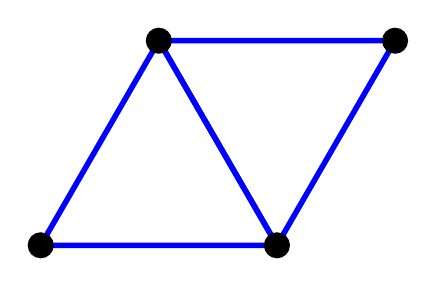
\begin{tikzpicture}[
  mesh/.style={gray},
  vertex/.style={circle, black, fill},
  facet/.style={blue, line width=2pt}]

\draw[mesh, facet] (0,0) -- ++(60:3) -- +(-60:3) -- cycle;
\draw[mesh, facet] (3,0) -- ++(60:3) -- +(-180:3) -- cycle;
\node[vertex] (v1) at (0,0) {};
\node[vertex] (v2) at (60:3) {};
\node[vertex] (v3) at (0:3) {};
\node[vertex] (v4) at ($(0:3) + (60:3)$) {};
\end{tikzpicture}
}

\only<4>{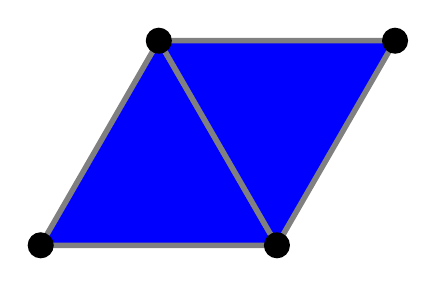
\begin{tikzpicture}[
  mesh/.style={gray, line width=2, fill=blue},
  vertex/.style={circle, black, fill}]

\draw[mesh] (0,0) -- ++(60:3) -- +(-60:3) -- cycle;
\draw[mesh] (3,0) -- ++(60:3) -- +(-180:3) -- cycle;
\node[vertex] (v1) at (0,0) {};
\node[vertex] (v2) at (60:3) {};
\node[vertex] (v3) at (0:3) {};
\node[vertex] (v4) at ($(0:3) + (60:3)$) {};
\end{tikzpicture}
}

\only<5>{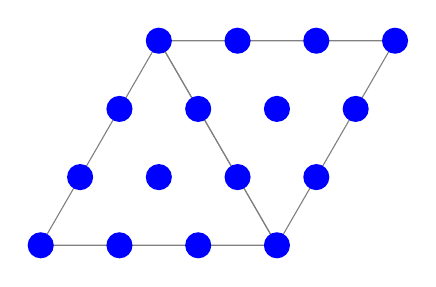
\begin{tikzpicture}[
  dof/.style={circle, blue, fill},
  mesh/.style={gray},
  vertex/.style={circle, blue, fill}]

\draw[mesh] (0,0) -- ++(60:3) -- +(-60:3) -- cycle;
\draw[mesh] (3,0) -- ++(60:3) -- +(-180:3) -- cycle;
\node[vertex] (v1) at (0,0) {};
\node[vertex] (v2) at (60:3) {};
\node[vertex] (v3) at (0:3) {};
\node[vertex] (v4) at ($(0:3) + (60:3)$) {};
\node[dof] (fd1) at (0:1) {};
\node[dof] (fd2) at (0:2) {};
\node[dof] (fd3) at (60:1) {};
\node[dof] (fd4) at (60:2) {};
\node[dof] (fd5) at ($(0:3) + (120:1)$) {};
\node[dof] (fd6) at ($(0:3) + (120:2)$) {};
\node[dof] (fd7) at ($(0:3) + (60:1)$) {};
\node[dof] (fd8) at ($(0:3) + (60:2)$) {};
\node[dof] (fd9) at ($(60:3) + (0:1)$) {};
\node[dof] (fd10) at ($(60:3) + (0:2)$) {};
\node[dof] (ed1) at (intersection cs: 
first line={(0,0)--(30:3)}, 
second line={(0:3)--($(0:3) + (150:3)$)}) {};
\node[dof] (ed2) at (intersection cs: 
first line={(0:3)--($(0:3) + (90:3)$)}, 
second line={(60:3)--($(60:3) + (-30:3)$)}) {};
\end{tikzpicture}
}
\par
\end{center}
\end{frame}

\begin{frame}[label={sec:orgheadline7}]{Data types II}
\begin{itemize}
\item \emph{Maps} between \emph{Sets}
\begin{itemize}
\item e.g. from elements to degrees of freedom
\end{itemize}
\item \emph{Dats}: data defined on a \emph{Set}
\item \emph{Kernels}
\begin{itemize}
\item code snippets to apply pointwise across \emph{Sets}
\end{itemize}
\item \emph{Sparsities} composed of outer products of pairs of \emph{Maps}
\begin{itemize}
\item give positions of non-zeros in discretisation of your operator
\end{itemize}
\item \emph{Mats}: data defined on a \emph{Sparsity}
\end{itemize}
\end{frame}

\begin{frame}[label={sec:orgheadline8}]{Iteration construct}
\begin{itemize}
\item \emph{par$\backslash$\(_{\text{loop}}\)}
\begin{itemize}
\item apply a \emph{Kernel} over every element in a \emph{Set}
\item access data in \emph{Dats} directly, or indirectly through \emph{Maps}
\end{itemize}
\item explicit access descriptors
\begin{itemize}
\item determination of concurrent writes, need for halo swaps can be
made by (simple) code
\end{itemize}
\end{itemize}
\end{frame}

\begin{frame}[label={sec:orgheadline9}]{Code generation targets}
\begin{itemize}
\item C (+ OpenMP) + MPI
\item CUDA (+ MPI [matrices not supported])
\item OpenCL (+ MPI [matrices not supported])
\end{itemize}
\end{frame}

\begin{frame}[fragile,label={sec:orgheadline10}]{Example application code}
 \begin{center}
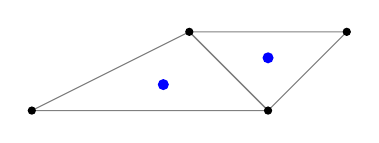
\begin{tikzpicture}[
  mesh/.style={gray},
  vertex/.style={circle, black, fill, inner sep=0pt, minimum size = 3pt},
centroid/.style={circle, blue, fill, inner sep=0pt, minimum size = 4pt}]

\draw[mesh] (0,0) -- (3,0) -- (2,1) -- cycle;
\draw[mesh] (3,0) -- (4,1) -- (2,1) -- cycle;
\node[vertex] (v1) at (0,0) {};
\node[vertex] (v2) at (3,0) {};
\node[vertex] (v3) at (2,1) {};
\node[vertex] (v4) at (4,1) {};

\node[centroid] (c1) at (1.67, 0.33) {};
\node[centroid] (c2) at (3, 0.67) {};
\end{tikzpicture}

\end{center}
\begin{minted}[frame=none,xleftmargin=1em,xrightmargin=1em,fontsize=\scriptsize,mathescape]{python}
vertices = Set(4)
cells = Set(2)
cell2vertex = Map(cells, vertices, 3, [0, 1, 2, 1, 2, 3])
coords = Dat(vertices, 2, [[0, 0], [3, 0], [2, 1], [4, 1]])
centroids = Dat(cells, 2, [[0, 0], [0, 0]])
centroid = Kernel("""void centroid(double *out, double *in[2]) {
        out[0] = (1.0/3.0) * (in[0][0] + in[1][0] + in[2][0]);
        out[1] = (1.0/3.0) * (in[0][1] + in[1][1] + in[2][1]);
                     }""", "centroid")
par_loop(centroid, cells, centroids(IdentityMap, WRITE),
         coords(cell2vertex, READ))
\end{minted}
\end{frame}

\begin{frame}[label={sec:orgheadline11}]{What happens under the hood}
\begin{itemize}
\item data structures recorded
\item par$\backslash$\(_{\text{loop}}\) encountered
\begin{itemize}
\item appropriate backend-specific code generated (cached for later use)
\item \ldots{} and executed
\item if necessary:
\begin{itemize}
\item MPI halo swaps performed
\item data uploaded to accelerator device
\end{itemize}
\end{itemize}
\end{itemize}
\end{frame}

\begin{frame}[label={sec:orgheadline12}]{Picture}
\begin{center}
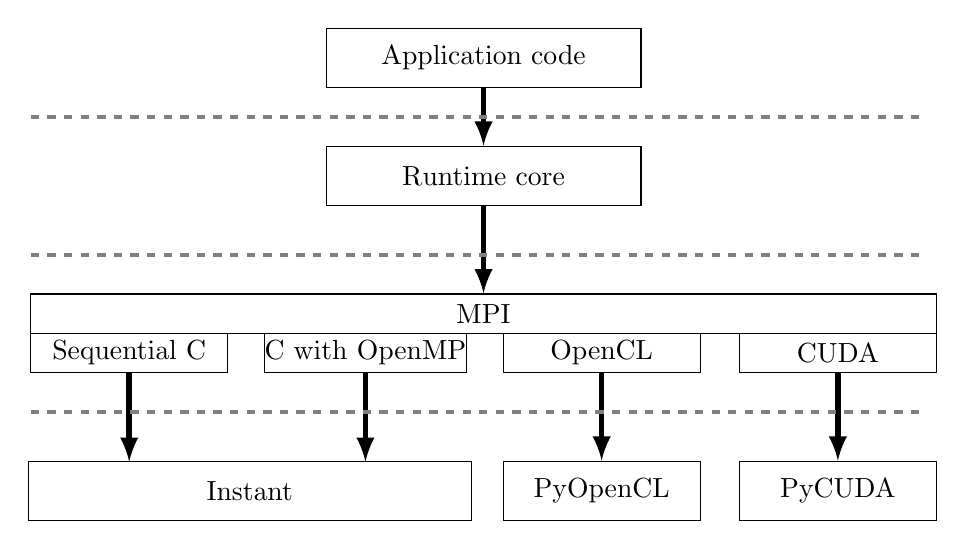
\begin{tikzpicture}[terminal/.style={draw, rectangle, 
 inner sep = 0pt, rounded corners=0mm, minimum height=0.75cm},
arrow/.style={-latex, draw, line width=2pt, black},
sep/.style={dashed, line width=1.5pt, gray}]


\node (user) at (0,0) [terminal, minimum width=4cm] {Application code};
\node (rt) at (0, -1.5) [terminal, minimum width=4cm] {Runtime core};

\node (mpi) at (0, -3.25) [terminal, minimum width=11.5cm, minimum height=0.5cm] {MPI};
\node (sc) at (-4.5, -3.75) [terminal, minimum width=2.5cm, minimum height=0.5cm] {Sequential C};
\node (oc) at (-1.5, -3.75) [terminal, minimum width=2.5cm, minimum height=0.5cm] {C with OpenMP};

\node (cl) at (1.5, -3.75) [terminal, minimum width=2.5cm, minimum height=0.5cm] {OpenCL};
\node (cu) at (4.5, -3.75) [terminal, minimum width=2.5cm, minimum height=0.5cm] {CUDA};

\node (instant) at (-2.97, -5.5) [terminal, minimum width=5.625cm] {Instant};
\node (pycl) at (1.5, -5.5) [terminal, minimum width=2.5cm] {PyOpenCL};
\node (pycu) at (4.5, -5.5) [terminal, minimum width=2.5cm] {PyCUDA};

\draw[arrow] (user) -- (rt);
\draw[arrow] (rt.south) -- (mpi.north);
% \draw[arrow] (rt.south) -- (cl.north);
% \draw[arrow] (rt.south) -- (cu.north);
\draw[arrow] (sc.south) -- +(0, -1.125);
\draw[arrow] (oc.south) -- +(0, -1.125);
\draw[arrow] (cl) -- (pycl);
\draw[arrow] (cu) -- (pycu);

\draw[sep] (-5.75, -0.75) -- (5.625, -0.75);
\draw[sep] (-5.75, -2.5) -- (5.625, -2.5);
\draw[sep] (-5.75, -4.5) -- (5.625, -4.5);

\end{tikzpicture}

\end{center}
\end{frame}

\section{Separating intent from implementation}
\label{sec:orgheadline20}

\begin{frame}[label={sec:orgheadline14}]{User/Runtime requirements}
\begin{itemize}
\item User defines
\begin{itemize}
\item execution, but not order
\item data (with specified input layout)
\item data access (isn't allowed to lie, otherwise they'll get
incorrect results)
\end{itemize}

\item Runtime library can
\begin{itemize}
\item choose to execute iteration in any order
\item choose to rearrange data (e.g. SoA vs. AoS)
\item split/fuse/reorder par$\backslash$\(_{\text{loops}}\)
\item as long as the result is correct
\end{itemize}
\end{itemize}
\end{frame}

\begin{frame}[label={sec:orgheadline15}]{As a result \ldots{}}
\begin{itemize}
\item we can rearrange data to be SoA on GPUs
\begin{itemize}
\item better memory coalescing
\end{itemize}
\item we can fuse user kernels (this is ``easy'' because we have explicit
data dependencies)
\item we can choose different representations of matrices
\begin{itemize}
\item e.g. fully or partially assembled, or matrix free [Markall
et al 2012 \url{doi:10.1002/fld.3648}]
\end{itemize}
\item \ldots{}
\end{itemize}
\end{frame}

\begin{frame}[label={sec:orgheadline16}]{\ldots{}}
\begin{itemize}
\item On GPUs, we explicitly manage shared memory cache
\item For shared memory parallelism (GPU + OpenMP on CPU)
\begin{itemize}
\item we can determine data dependencies and avoid race conditions
\item cache block if appropriate
\end{itemize}
\item Determine when halo swaps are required on distributed memory
systems
\end{itemize}
\end{frame}

\begin{frame}[label={sec:orgheadline17}]{Performance}
\begin{itemize}
\item Runtime library used to replace FE advection-diffusion solver in
Fluidity's dynamical core
\begin{itemize}
\item use FEniCS code generation technology for elementary kernel
\end{itemize}
\item Code runs faster in serial (maintains advantage in MPI parallel)
\item Taking advantage of GPUs: one line change in source code.
\end{itemize}
\end{frame}

\begin{frame}[label={sec:orgheadline18}]{Test case}
\begin{itemize}
\item 2D Advection-diffusion, P1 Lagrange elements, 100 timesteps
\item Compare Fluidity builtin support with PyOP2 on various backends
\item CPU: 12 core Westmere; GPU: C2050
\end{itemize}
\begin{center}
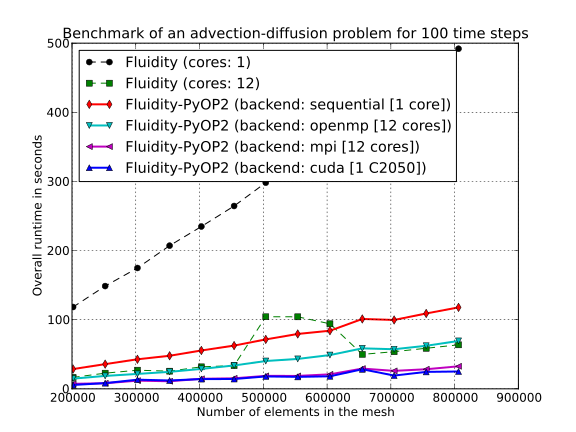
\includegraphics[height=0.7\textheight]{04-11-EASC-PyOP2-fluidity.figures/runtime_linear}
\end{center}
\end{frame}

\begin{frame}[fragile,label={sec:orgheadline19}]{How much code?}
 \begin{itemize}
\item Fluidity
\end{itemize}
\begin{minted}[frame=none,xleftmargin=1em,xrightmargin=1em,fontsize=\scriptsize,mathescape]{fortran}
1500 lines of fortran elided
\end{minted}
\begin{itemize}
\item PyOP2 (using FEniCS to generate kernel code)
\end{itemize}
\begin{minted}[frame=none,xleftmargin=1em,xrightmargin=1em,fontsize=\scriptsize,mathescape]{python}
t = state.scalar_fields["Tracer"]
u = state.vector_fields["Velocity"]
p = TrialFunction(t)
q = TestFunction(t)
diffusivity = 0.1
M = p*q*dx
d = dt*(diffusivity*dot(grad(q),grad(p)) - dot(grad(q),u)*p)*dx
a = M + 0.5*d
L = action(M - 0.5*d, t)
solve(a == L, t)
\end{minted}
\end{frame}
\section{Conclusions}
\label{sec:orgheadline24}

\begin{frame}[label={sec:orgheadline21}]{Conclusions}
\begin{itemize}
\item Given a suitably constrained domain
\begin{itemize}
\item it's possible to automatically generate performance-portable code
\end{itemize}
\item many optimisations possible that would be incredibly difficult to do
by hand (and if possible, highly unmaintainable)
\item writing code is less error-prone
\item your application code is better able to cope with changing hardware
\end{itemize}
\end{frame}

\begin{frame}[label={sec:orgheadline22}]{Future work}
\begin{itemize}
\item Matrix-free application of FE operators
\scriptsize [Kirby and Kieu, Numerische Mathematik 121(2):261 (2012), Ainsworth
et al SIAM JSC 33(6):3087 (2011)]
\begin{itemize}
\item turns sparse LA into application of dense
blocks + gather/scatter
\end{itemize}

\item Lazy evaluation (e.g. postponing halo swap completion as late as possible)

\item 2d unstructured + 1d structured (for ocean/climate)
\begin{itemize}
\item currently under development at IC
\end{itemize}
\end{itemize}
\end{frame}

\begin{frame}[label={sec:orgheadline23}]{Thanks}
\begin{itemize}
\item Code is available (BSD license)
\begin{itemize}
\item \url{http://github.com/OP2/PyOP2}
\item \url{http://www.oerc.ox.ac.uk/research/op2}
\end{itemize}
\item Funding
\begin{itemize}
\item MAPDES (EPSRC grants EP/I00677X/1, EP/I006079/1)
\item APOS-EU (EU FP7/277481)
\end{itemize}
\end{itemize}
\end{frame}
\end{document}
